\chapter{插值与拟合}
\begin{introduction}
\item 插值与插值函数
\item interp1,spline,pchip
\item 拟合与拟合函数
\item regress、ployfit、nlinfit
\end{introduction}
\section{插值函数的基本概念}
\subsection{插值函数}
\begin{definition}{插值函数}{}
a)插值函数$\phi(x)$近似于原函数$f(x)$
\[
y=f(x)\approx\phi(x)
\]

b)在插值点$x_i$处,插值函数值$\phi(x_i)$等于原函数值$f(x_i)$
\[
\phi(x_i)=f(x_i)=y_i
\]
\end{definition}

常见形式有:

\textbf{拉格朗日多项式插值、分段三次埃米特插值、分段三次样条插值...}
\subsection{拉格朗日插值法}
\begin{definition}{拉格朗日插值法}{}
拉格朗日n次插值多项式:
\[
P_n(x)=\sum_{i=0}^{n}{y_iL_i(x)}
\]
需要(n+1)个样本点,为了实现
\[P_n(x_i)=y_i\]
我们让基函数$L_i(x)$满足
\[L_i(x)=
\begin{cases}
1 & \text{if } x=x_i\\
0 & \text{if } x\neq x_i
\end{cases} \]
我们令
\[
L_i(x)=\prod_{\substack{j=0\\j\neq i}}^{n}\frac{x-x_j}{x_i-x_j}
\]
即为基函数定义。
\end{definition}

Lagrange插值多项式的优点在于不要求数据点是等间隔的,其缺点是数据点数不宜过大,通常不超过7个,否则计算工作量大且误差大,计算不稳定。

\begin{definition}{龙格现象}{}
当次数n增大时,部分区间上误差严重,这种现象称“龙格现象”。

[解决方法]:分段插值。
\end{definition}

\begin{note}
拉格朗日插值多项式次数高,不等于插值效果好!
\end{note}
\subsection{三次样条插值}
需要知道:区间$[a,b]$内节点$x_i$处函数值$y_i$,以及端点附近导数值等。
\begin{definition}{样条插值函数$S(x)$}{}
满足条件:

a)$S(x)$在分段区间$[x_i,x_{i+1}]$上为三次多项式

b)$S(x)$、$S'(x)$、$S''(x)$在$[a,b]$上连续

c)节点处$S(x)=y_i$

\end{definition}
\begin{note}
[自然边界条件\footnote{我的理解是:可在边界附近有较好的单调性。}]
:\quad $S''(x_0)=S''(x_n)=0$
\end{note}

\subsection{分段三次埃米特插值}
需要知道:$x_i$处的函数值$y_i$和导数值$y_i'$。
\begin{definition}{Hermite插值函数$H(x)$}{}
a)每个插值区间上H(x)为三次多项式

b)插值函数值等于节点值
\[H(x_i)=y_i
\]
c)插值函数一阶导数等于节点处导数值
\[H'(x_i)=y_i'
\]
\end{definition}

\begin{note}
二者不同之处在于一阶导数的确定方法不同。
其中,埃米特插值可保持函数形状。
\end{note}

\newpage

\section{MATLAB中的插值函数}
\subsection{interp1函数}
\begin{lstlisting}[frame=single,numbers=left]
% 调用格式
yi=interp1(x,y,xi,’`\mlplaceholder{method}`’)
% x,y为样本数据,xi为插值点
% `\mlplaceholder{method}`省略时默认线性插值
% `\mlplaceholder{method}`可选:
% 最近插值nearest、埃米特插值pchip、样条插值spline
\end{lstlisting}

\subsection{pichp函数与spline函数}\label{spline}
\begin{lstlisting}[frame=single,numbers=left]
% 调用格式
% 插值函数值
yi=pchip(x,y,xi)
% 插值函数
pp=pchip(x,y)
% spline函数使用方式相同,从略
\end{lstlisting}

以下三种调用形式结果相同:
\begin{lstlisting}[frame=single,numbers=left]
y1=interp1(x,y,xi,'pchip')
\end{lstlisting}
\begin{lstlisting}[frame=single,numbers=left]
yi=pchip(x,y,xi)
\end{lstlisting}
\begin{lstlisting}[frame=single,numbers=left]
pp=pchip(x,y);
yi=fnval(pp,xi)
\end{lstlisting}

\begin{note}
可以参考\ref{fnval}中的关于函数fnval的介绍,应用见\ref{cubic}。
\end{note}

\newpage
\section{拟合函数的基本概念}
\textcolor{third}{\textbf{拟合函数}}\textbf{不要求}函数完全通过数据点,常用方法为\textbf{最小二乘法}。

\begin{definition}{最小二乘法}{}
[原理]

近似函数在各实验点的计算结果与实验结果的偏差平方和最小。

[线性最小二乘]

可通过解方程组得到拟合函数。

[非线性最小二乘]

a)线性化;

b)直接迭代。
\end{definition}
\section{MATLAB中的拟合函数}\label{fit}
\subsection{ployfit函数}
polyfit是MATLAB的\textcolor{third}{\textbf{多项式拟合}}函数。
\begin{lstlisting}[frame=single,numbers=left]
% 调用格式
p=polyfit(x,y,n)
% x,y为样本,n为多项式次数
\end{lstlisting}

常与polyval联合使用,计算指定点的值:
\begin{lstlisting}[frame=single,numbers=left]
% 调用格式
yy=polyval(p,xx)
\end{lstlisting}

\begin{note}
此处p定义与roots函数\ref{ployp}中相同,请对照理解。
\end{note}
\subsection{regress函数}
regress是MATLAB的\textcolor{third}{\textbf{多元线性拟合 }}函数。
\begin{lstlisting}[frame=single,numbers=left]
% 调用格式
b=regress(y,x)
% n个自变量xi,进行m次实验,得到m次结果yi
% y为m行1列向量
% x为m行n列矩阵
\end{lstlisting}

\begin{note}
可以拟合线性化后的非线性函数。
\end{note}

\newpage

\begin{problem}\label{problemRegress}
已知x1=1:6,x2=1.5:0.2:2.5,y=[5.9512 10.6730 15.5676 20.6234 25.8599 31.2622]。试编写函数,采用以上数据拟合y=a*x1+b*x2+c*x1\^{}2+d*x1*x2中的系数\footnote{摘自隋志军老师课件W09}。
\end{problem}

\begin{solution}
将x1,x2,x1\^{}2和x1*x2视为自变量,则以上的拟合为多元线性拟合,可以采用regress函数求解。
\begin{lstlisting}
function LinearFitting
x1=1:6;
x2=1.5:0.2:2.5;
y=[5.9512 10.6730 15.5676 20.6234 25.8599 31.2622];
X=[x1;x2;x1.^2;x1.*x2];
% 关键函数
% 注意按照列的形式输入
b=regress(y',X') %结果为[0;1.0775;-0.5687;3.2694],即[a;b;c;d]
\end{lstlisting}

可进一步作图观察拟合结果:
\begin{lstlisting}
bb=repmat(b,1,6);
yi=sum(bb.*X);
plot(x1,y,'rp',x1,yi,'bo')
legend('原始数据','拟合数据')
\end{lstlisting}

\begin{figure}[htbp]
\centering
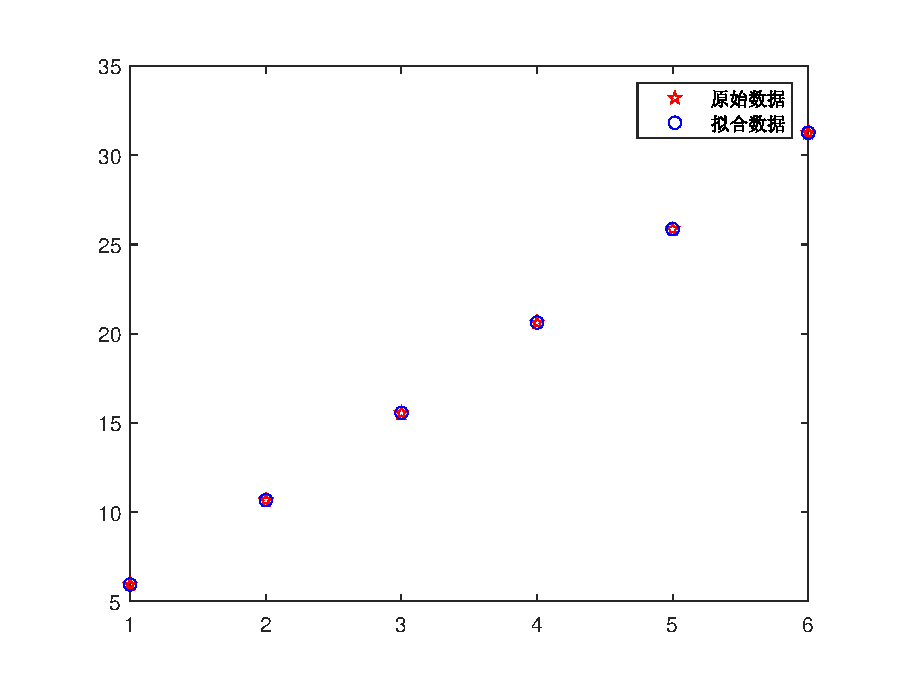
\includegraphics[width=0.8\textwidth]{regress.eps}
\caption{regress拟合效果图}
\end{figure}
\end{solution}

\newpage

\subsection{nlifit函数}
\begin{lstlisting}[frame=single,numbers=left]
beta=nlinfit(x,y,fun,beta0)
% x,y用法与regress函数类似
% fun可为匿名函数或函数句柄
% beta0是回归系数初值,beta为估计出的回归系数
\end{lstlisting}

\begin{note}
非线性方程建议采用直接非线性最小二乘法拟合,fun调用可参考\ref{func}。
\end{note}

\begin{problem}
用nlifit函数求解例题\ref{problemRegress}:
\end{problem}

\begin{solution}
\begin{lstlisting}
function NonLinearFitting
x1=1:6;
x2=1.5:0.2:2.5;
y=[5.9512 10.6730 15.5676 20.6234 25.8599 31.2622];
beta0=[0 0 0 0];%对结果影响较大
% 关键函数
beta=nlinfit([x1',x2'],y',@fun,beta0) %与初值选取有关
% 验证结果
yi=fun(beta,[x1',x2']); %拟合函数在样本处点的函数值
plot(x2,y,'ro',x2',yi,'bp') %作图对比
errMax=max(abs(y'-yi)) %最大偏差为0.0034,与regress相同

%拟合函数部分
function y=fun(Beta,x)
a=Beta(1);b=Beta(2);c=Beta(3);d=Beta(4); %提高代码可读性
x1=x(:,1);x2=x(:,2); %与上一行本质上可以略去,不过下一行会比较复杂
y=a*x1+b*x2+c*x1.^2+d*x1.*x2;
\end{lstlisting}
\end{solution}
\newpage
\subsection{csaps函数}\label{fnval}
\begin{lstlisting}[frame=single,numbers=left]
% Cubic smoothing spline 平滑三次样条拟合函数
% 拟合函数
pp=csaps(x,y,p,[],w)
% p:平滑参数,范围[0,1],默认为1,即spline
% w:误差权重,默认为1
% 拟合函数值
values=csaps(x,y,p,xx,w)
\end{lstlisting}

\begin{lstlisting}[frame=single,numbers=left]
pp=csaps(x,y,p,[],w);
values=fnval(pp,xx) 
% 函数fnval
fnval(f,x) %计算函数f在x处的函数值
\end{lstlisting}

\begin{note}
可以参考\ref{spline}中的相关介绍。
\end{note}